% MD_en_Haskell.tex
% Matemática discreta (MD) en Haskell.
% María Dolores Valverde Rodríguez
% Sevilla, 16 de julio de 2016
% =============================================================================

\documentclass[a4paper,12pt,twoside]{book}

%%%%%%%%%%%%%%%%%%%%%%%%%%%%%%%%%%%%%%%%%%%%%%%%%%%%%%%%%%%%%%%%%%%%%%%%%%%%%%
%%  Paquetes adicionales                                                   %%
%%%%%%%%%%%%%%%%%%%%%%%%%%%%%%%%%%%%%%%%%%%%%%%%%%%%%%%%%%%%%%%%%%%%%%%%%%%%%%

\usepackage[utf8x]{inputenc}       % Acentos de UTF8
\usepackage[spanish]{babel}        % Castellanización.
\usepackage[T1]{fontenc}           % Codificación T1 con European Computer
                                   % Modern.  
\usepackage{graphicx}
\usepackage{fancyvrb}              % Verbatim extendido
\usepackage{makeidx}               % Índice
\usepackage{amsmath}               % AMS LaTeX
\usepackage{amsthm} 
\usepackage{latexsym}
\usepackage[colorinlistoftodos
           , backgroundcolor = yellow
           , textwidth = 4cm
           , shadow
           , spanish]{todonotes}

% Fuentes
\usepackage{mathpazo}              % Fuentes semejante a palatino
\usepackage[scaled=.90]{helvet}
\usepackage{cmtt}
\renewcommand{\ttdefault}{cmtt}
\usepackage{a4wide}
% \usepackage{xmpincl}               % Incluye metadato de licencia CC.

% Tikz
\usepackage{tkz-berge}
% Desactivar <,> cuando se hacen dibujos con tikz.
\tikzset{
every picture/.append style={
  execute at begin picture={\deactivatequoting},
  execute at end picture={\activatequoting}
  }
}

% Márgenes
\usepackage[margin=1in]{geometry}

% Control de espacios en la tabla de contenidos:
\usepackage[titles]{tocloft}
\setlength{\cftbeforechapskip}{2ex}
\setlength{\cftbeforesecskip}{0.5ex}
\setlength{\cftsecnumwidth}{12mm}
\setlength{\cftsubsecindent}{18mm}

% Control de listas
% Elimina espacio entre item y párrafo y coloca item en el margen izquierdo
\usepackage{enumitem}
\setlist[enumerate,itemize]{noitemsep, nolistsep, leftmargin=*}

\usepackage{minitoc}

% Doble espacio entre líneas
\usepackage{setspace}
\onehalfspacing

% \linespread{1.05}                % Distancia entre líneas
\setlength{\parindent}{5mm}        % Indentación de comienzo de párrafo
\deactivatetilden                  % Elima uso de ~ para la eñe
\raggedbottom                      % No ajusta los espacios verticales.

\usepackage[%
  pdftex,
  pdfauthor={Maria Dolores Valverde},%
  pdftitle={MD en Haskell},%
  pdfstartview=FitH,%
  bookmarks=false,%
  colorlinks=true,%
  urlcolor=blue,%
  unicode=true]{hyperref} 
     
\usepackage{caption} % Personalizar leyendas y notas al pie

%%%%%%%%%%%%%%%%%%%%%%%%%%%%%%%%%%%%%%%%%%%%%%%%%%%%%%%%%%%%%%%%%%%%%%%%%%%%%%
%%  Cabeceras                                                              %%
%%%%%%%%%%%%%%%%%%%%%%%%%%%%%%%%%%%%%%%%%%%%%%%%%%%%%%%%%%%%%%%%%%%%%%%%%%%%%%

\usepackage{fancyhdr}

\addtolength{\headheight}{\baselineskip}

\pagestyle{fancy}

\cfoot{}

\fancyhead{}
\fancyhead[RE]{\bfseries \nouppercase{\leftmark}}
\fancyhead[LO]{\bfseries \nouppercase{\rightmark}}
\fancyhead[LE,RO]{\bfseries \thepage}

%%%%%%%%%%%%%%%%%%%%%%%%%%%%%%%%%%%%%%%%%%%%%%%%%%%%%%%%%%%%%%%%%%%%%%%%%%%%%%
%%  Definiciones                                                           %%
%%%%%%%%%%%%%%%%%%%%%%%%%%%%%%%%%%%%%%%%%%%%%%%%%%%%%%%%%%%%%%%%%%%%%%%%%%%%%%

\input definiciones
\def\mtctitle{Contenido}

%%%%%%%%%%%%%%%%%%%%%%%%%%%%%%%%%%%%%%%%%%%%%%%%%%%%%%%%%%%%%%%%%%%%%%%%%%%%%%
%%  Título                                                                 %%
%%%%%%%%%%%%%%%%%%%%%%%%%%%%%%%%%%%%%%%%%%%%%%%%%%%%%%%%%%%%%%%%%%%%%%%%%%%%%%

\title{\Huge Matemática discreta en Haskell}
\author{María Dolores Valverde Rodríguez}
\date{\vfill \hrule \vspace*{2mm}
  \begin{tabular}{l}
      \href{http://www.cs.us.es/glc}
           {Grupo de Lógica Computacional} \\
      \href{http://www.cs.us.es}
           {Dpto. de Ciencias de la Computación e Inteligencia Artificial} \\
      \href{http://www.us.es}
           {Universidad de Sevilla}  \\
      Sevilla, 21 de junio de 2016 (Versión de \today)
  \end{tabular}\hfill\mbox{}}


%%%%%%%%%%%%%%%%%%%%%%%%%%%%%%%%%%%%%%%%%%%%%%%%%%%%%%%%%%%%%%%%%%%%%%%%%%%%%%%
%%  Construcción del índice                                                 %%
%%%%%%%%%%%%%%%%%%%%%%%%%%%%%%%%%%%%%%%%%%%%%%%%%%%%%%%%%%%%%%%%%%%%%%%%%%%%%%%

\makeindex

%%%%%%%%%%%%%%%%%%%%%%%%%%%%%%%%%%%%%%%%%%%%%%%%%%%%%%%%%%%%%%%%%%%%%%%%%%%%%%
%%  Documento                                                              %%
%%%%%%%%%%%%%%%%%%%%%%%%%%%%%%%%%%%%%%%%%%%%%%%%%%%%%%%%%%%%%%%%%%%%%%%%%%%%%%

% \includeonly{Programacion_funcional_con_Haskell}

% \includexmp{licencia}

\begin{document}
\dominitoc

\begin{titlepage}
 \vspace*{2cm}
  \begin{center}
    {\huge \textbf{Matemática discreta en Haskell}}
  \end{center}
  \vspace{3cm}
  \begin{center}
    \begin{figure}[h]
    \centering
    \includegraphics[scale=.3]{fig/sello}
    \end{figure}
  \vspace{3cm}
    {\normalsize Facultad de Matemáticas} \\
    {\normalsize Departamento de Ciencias de la Computación e Inteligencia Artificial}\\
    {\normalsize Trabajo Fin de Grado} \\
  \end{center}
  \begin{center}
    {\large \textbf{María Dolores Valverde Rodríguez}}
  \end{center}
\end{titlepage}

\newpage

\noindent
Esta obra está bajo una licencia Reconocimiento--NoComercial--CompartirIgual
2.5 Spain de Creative Commons. 

\vspace*{4ex}

\begin{center}
\fbox{
\begin{minipage}{175mm}
\vspace*{1ex}
\noindent                     
{\bf Se permite:}
\begin{itemize}                         
\item copiar, distribuir y comunicar públicamente la obra
\item hacer obras derivadas
\end{itemize}
         
\noindent       
{\bf Bajo las condiciones siguientes:}

\begin{minipage}[t]{20mm}
  \vspace*{0mm}\hspace*{1em}
  
\includegraphics[scale=0.35]{deed.png}
\end{minipage}%
\begin{minipage}[t]{15cm}
  \vspace*{0mm}
  {\bf Reconocimiento}. Debe reconocer los créditos de la  obra de la manera
  especificada por el autor.  
\end{minipage}
\\[1ex]

\begin{minipage}[t]{20mm}
  \vspace*{0mm}\hspace*{1em}
  
\includegraphics[scale=0.35]{deed-eu.png}
\end{minipage}%
\begin{minipage}[t]{15cm}
  \vspace*{2mm}
  {\bf No comercial}. No puede utilizar esta obra para fines comerciales.
\end{minipage}
\\[1ex]

\begin{minipage}[t]{20mm}
  \vspace*{0mm}\hspace*{1em}
  
\includegraphics[scale=0.35]{deed_002.png}
\end{minipage}%
\begin{minipage}[t]{15cm}
  \vspace*{-2mm}
  {\bf Compartir bajo la misma licencia}. Si altera o transforma esta obra, o
  genera una obra derivada, sólo puede distribuir la obra generada bajo una
  licencia idéntica a ésta. 
\end{minipage}

\begin{itemize}    
\item Al reutilizar o distribuir la obra, tiene que dejar bien claro los
  términos de la licencia de esta obra. 
\item Alguna de estas condiciones puede no aplicarse si se obtiene el permiso
 del titular de los derechos de autor.
\end{itemize}
\vspace*{1ex}
\end{minipage}}
\end{center}

\vspace*{4ex}

Esto es un resumen del texto legal (la licencia completa). Para ver una copia
de esta licencia, visite 
\href{http://creativecommons.org/licenses/by-nc-sa/2.5/es/}
     {\url{http://creativecommons.org/licenses/by-nc-sa/2.5/es/}}
o envie una carta a Creative Commons, 559 Nathan Abbott Way, Stanford,
California 94305, USA.

%%% Local Variables: 
%%% mode: latex
%%% TeX-master: t
%%% End: 

\newpage 

\tableofcontents
\newpage

\chapter*{Agradecimientos}
\addcontentsline{toc}{chapter}{Agradecimientos}

Quisiera agradecer a todas las personas que me han apoyado y prestado
sus conocimientos a lo largo de estos cuatro años del grado. Gracias a ellos, 
el esfuerzo ha merecido la pena.

En primer lugar, me gustaría destacar a María José Hidalgo Doblado y José 
Antonio Alonso Jiménez, mi tutores en este Trabajo de Fin de Grado. Les
agradezco de todo corazón la constancia y la atención que me han brindado 
a pesar de las dificultades que supone realizar el proyecto durante un curso
curso en el que estoy disfrutando la oportunidad de la movilidad internacional
Erasmus. Son para mí un referente y un claro ejemplo de lo que se puede 
conseguir con esfuerzo y trabajo en equipo.

Seguidamente, expresar mi gratitud al resto de profesores y trabajadores
de la Universidad de Sevilla, especialmente a aquellos que se esfuerzan 
por mejorar la institución día a día.

Quiero agradecer también este trabajo a mi familia, en especial a mis padres,
que me apoyaron desde el principio cuando tomé la decisión de cambiar de
carrera y siempre han intentado brindarnos a mi hermana y a mí con lo mejor.

Finalmente a mis amigos y compañeros, que han hecho de esta primera etapa 
universitaria un capítulo de mi vida lleno de bonitos recuerdos. En especial
a Pedro, con el que he compartido tantas horas de estudio y trabajo.

Muchas gracias a todos.

\chapter*{Abstract}
\addcontentsline{toc}{chapter}{Abstract}

Discrete mathematics is characterized as the branch of mathematics
dealing with finite and numerable sets. Concepts and notations from
discrete mathematics are useful in studying and describing objects 
and real-life problems. In particular the graph theory has numerous
applications in logistics.


Throughout this project some of the knowlegde adquired from the course
``Matemática Discreta'' will be given a computational implementation.
The code will be written in Haskell language and a free version of it 
will be available in GitHub under the name: \textit{MDenHaskell}.
The work will focus on the graph theory and will provide some
examples and algorithms in order to give an introduction of it and how
it can be implemented in Haskell. 

At first, two chapters will be presented as a gentle reminder of basic
concepts related to the set theory and the relations that can be established
among them. The third chapter will introduce the main topic, graph theory,
with different representations, definitions and examples on graphs. It will
go through aspects such as morphism, connectivity and paths in graphs. Finally
some properties and advantages of working with adjacency matrices will be 
presented in the fourth chapter.

This project leaves the door open for the community of programmers
to continue and improve it. It can be used as a self-learning tool
as well as to make calculations that by hand would be tedious.

\chapter*{Introducción}
\addcontentsline{toc}{chapter}{Introducción}

El objetivo del trabajo es la implementación de algoritmos de Matemática
Discreta en Haskell. Los puntos de partida son 
\begin{itemize}
\item los temas de la asignatura
\href{https://dl.dropboxusercontent.com/u/15420416/tiddly/emptyMD1314.html}
     {Matemática discreta}\
\footnote{\url{https://dl.dropboxusercontent.com/u/15420416/tiddly/emptyMD1314.html}}
(\cite{Cardenas-15a})

\item los temas de la asignatura 
\href{https://www.cs.us.es/~jalonso/cursos/i1m-15}
     {Informática}\
\footnote{\url{{https://www.cs.us.es/~jalonso/cursos/i1m-15}}}
(\cite{Alonso-15a}) 

\item el capítulo 7 del libro 
\href{http://www.iro.umontreal.ca/~lapalme/Algorithms-functional.html}
     {Algorithms: A functional programming approach}\
\footnote{\url{http://www.iro.umontreal.ca/~lapalme/Algorithms-functional.html}}
(\cite{Rabhi+Lapalme-99}) y

\item el artículo
\href{https://en.wikipedia.org/wiki/Graph_theory}
     {Graph theory}\
\footnote{\url{https://en.wikipedia.org/wiki/Graph_theory}}
(\cite{Wikipedia-grafos}) de la Wikipedia.  

\end{itemize}
 
%%% Local Variables: 
%%% mode: latex
%%% TeX-master: "MD_en_Haskell"
%%% End: 

\chapter{Conjuntos}

El concepto de \textit{conjunto} aparece en todos los campos de las
Matemáticas, pero, ¿qué debe entenderse por él? La \textit{Teoría de conjuntos}
fue introducida por Georg Cantor (1845-1917); desde 1869, Cantor ejerció como
profesor en la Universidad de Halle y entre 1879 y 1884 publicó una serie de
seis artículos en el \textit{Mathematische Annalen}, en los que hizo una
introducción básica a la teoría de conjuntos. En su \textit{Beiträge zur
Begründung der transfiniten Mengenlehre}, Cantor dio la siguiente definición
de conjunto:

\begin{figure}[h]
  \centering
  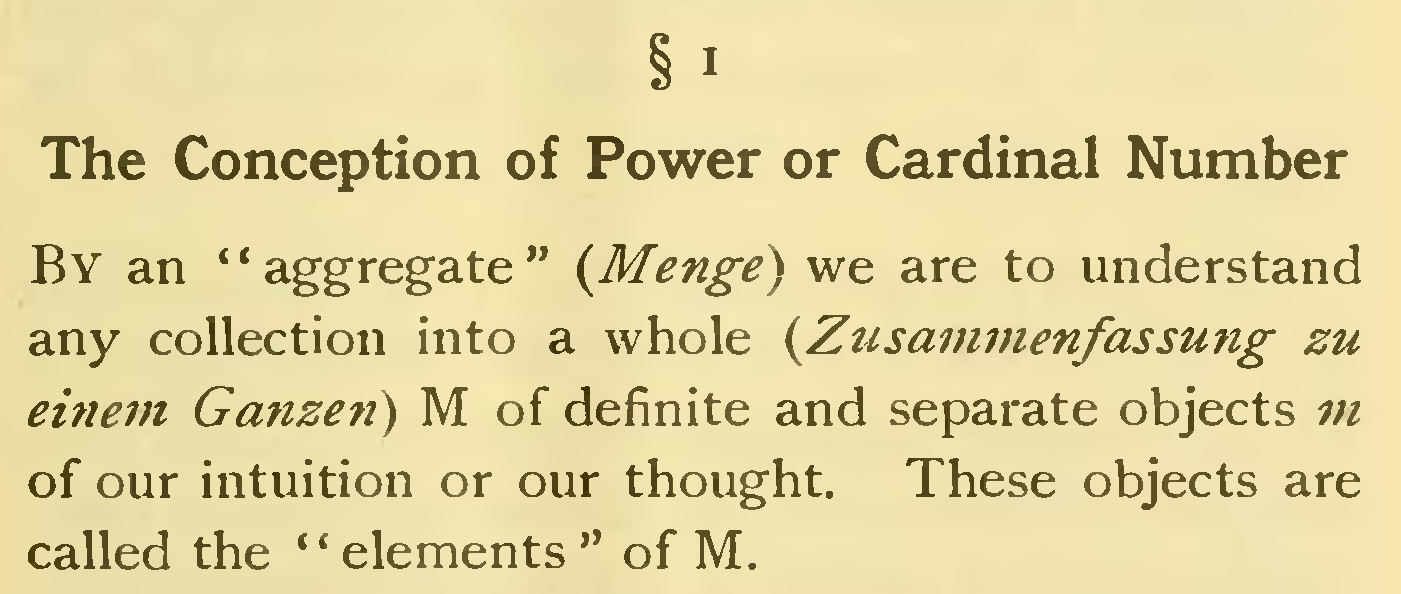
\includegraphics[scale=.2]{fig/definicionConjunto}
  \captionsetup{font=footnotesize}
  \caption{Fragmento del texto traducido al inglés en el que Cantor da la
    definición de conjunto}
\end{figure}

\begin{quote}
  <<Debemos entender por ``conjunto'' (\textit{Menge}) cualquier colección
  vista como un todo (Zusammenfassung zu einem Ganzen), $M$, de objetos
  separados y bien definidos, $m$, de nuestra intuición o pensamiento. Estos
  objetos son los ``elementos'' de $M$>>
\end{quote}

Felix Hausdorff, en 1914, dice: <<un conjunto es una reunión de cosas que
constituyen una totalidad; es decir, una nueva cosa>>, y añade: <<esto puede
difícilmente ser una definición, pero sirve como demostración expresiva del
concepto de conjunto a través de conjuntos sencillos como el conjunto de
habitantes de una ciudad o el de átomos de Hidrógeno del Sol>>.

Un conjunto así definido no tiene que estar compuesto necesariamente de
elementos homogéneos y además, da lugar a cuestiones filosóficas como si
podemos llamar \textit{conjunto} a aquel que no posee ningún elemento.
Matemáticamente, conviene aceptar solo elementos que compartan alguna propiedad
y definir el \textit{conjunto vacío} como aquel que no tiene elemento alguno.

El gran mérito de Cantor fue considerar conjuntos \textit{transfinitos} (que
tiene infinitos elementos), concepto inaudito hasta avanzado el siglo XIX,
hablar del \textit{cardinal} de un conjunto como el número de sus elementos y
hablar de \textit{conjuntos equivalentes} cuando puede establecerse una
biyección entre ellos; ideas ya apuntadas por Bolzano, quien se centró
demasiado en el aspecto filosófico, sin llegar a formalizar sus ideas.\\


A lo largo de la sección, haremos una pequeña introducción a la Teoría de
Conjuntos, presentando formalmente sus conceptos más importantes. A la hora de 
elaborar el contenido se han utilizado los siguientes recursos bibliográficos:

\begin{itemize}
\item[$*$] el primer tema de la asignatura
\href{https://rodas5.us.es/file/19961ac2-66e4-4af4-bf13-81f29b771a1b/1/01-Conjuntos.pdf}
     {Álgebra Básica}\
\footnote{\url{https://rodas5.us.es/file/19961ac2-66e4-4af4-bf13-81f29b771a1b/1/01-Conjuntos.pdf}}
(\cite{Algebra-15a})

\item[$*$] los temas de la asignatura 
\href{https://www.cs.us.es/~jalonso/cursos/i1m-15}
     {Informática}\
\footnote{\url{{https://www.cs.us.es/~jalonso/cursos/i1m-15}}}
(\cite{Alonso-15a}) 
 
\item[$*$] el artículo de la Wikipedia
\href{https://en.wikipedia.org/wiki/Set_(mathematics)}
     {Set (mathematics)}\
\footnote{\url{https://en.wikipedia.org/wiki/Set_(mathematics)}}
(\cite{Wikipedia-grafos}) y

\item[$*$] el artículo
\href{http://catedu.es/materranya/suplemento3.pdf}
     {\textit{El regalo de Cantor}}\
\footnote{http://catedu.es/materranya/suplemento3.pdf}
\end{itemize}

\section{El TAD de los conjuntos}

\label{sec:TAD_conjuntos}

En la presente sección, se defininen las operaciones básicas necesarias
para trabajar con conjuntos en un lenguaje funcional. En nuestro caso, 
el lenguaje que utilizaremos será Haskell. Daremos la signatura del Tipo
Abstracto de Dato (TAD) de los conjuntos y daremos algunos ejemplos de 
posibles representaciones de conjuntos con las que podríamos trabajar.

A continuación, presentamos las operaciones definidas en el TAD de los 
conjuntos:

\begin{code}
vacio          :: Conj a                         
inserta        :: Eq a => a -> Conj a -> Conj a
elimina        :: Eq a => a -> Conj a -> Conj a
pertenece      :: Eq a => Conj a -> a -> Bool  
esVacio        :: Conj a -> Bool
minimoElemento :: Ord a => Conj a -> a
\end{code}

donde,

\begin{itemize}
\item \texttt{(vacio)} es el conjunto vacío.
\item \texttt{(inserta x c)} es el conjunto obtenido añadiendo el      
      elemento \texttt{x} al conjunto \texttt{c}.
\item \texttt{(elimina x c)} es el conjunto obtenido eliminando el
      elemento \texttt{x} del conjunto \texttt{c}.
\item \texttt{(pertenece x c)} se verifica si \texttt{x} pertenece al
      conjunto \texttt{c}.
\item \texttt{(esVacio c)} se verifica si \texttt{c} no tiene ningún
      elemento.
\item \texttt{(minimoElemento c)} devuelve el mínimo elemento del      
      conjunto \texttt{c}.\\
\end{itemize}


Hemos de tener en cuenta que a la hora de crear un nuevo tipo de dato 
con el que representar a los conjuntos, este debe ser compatible con 
la entidad matemática que representa.\\

Estas son algunas de las posibles representaciones con las que podríamos
trabajar con conjuntos en Haskell:

\begin{itemize}
  \item[-] en primer lugar, podemos trabajar con la librería  
        \texttt{Data.Set}; en este caso, la implementación del tipo de 
        dato \texttt{Set} está basado en árboles binarios balanceados.
  \item[-] Por otra parte, podemos definir un nuevo tipo \texttt{Cj xs} con  
        el que trabajar con conjuntos como listas no ordenadas con        
        duplicados, como listas no ordenadas sin duplicados o como        
        listas ordenadas sin duplicados.
  \item[-] Otra opción sería trabajar directamente con conjuntos como  
        listas, para ello, debemos cuidar que las listas no tengan        
        duplicados.
  \item[-] Los conjuntos que sólo contienen números (de tipo \texttt{Int)} 
        entre $0$ y $n-1$, se pueden representar como números binarios 
        con $n$ bits donde el bit $i (0 ≤ i < n)$ es $1$ syss el número
        $i$ pertenece al conjunto.
\end{itemize}

\begin{nota}
  Las funciones que aparecen en la especificación del TAD no dependen 
  de la representación que elijamos.
\end{nota}

\subsection{Conjuntos como listas ordenadas sin repetición}

\entrada{ConjuntosConListasOrdenadasSinRepeticion}

\section{Definiciones y operaciones}

\entrada{DefinicionesYPropiedadesConjuntos}

\chapter{Relaciones y funciones}

\section{Relaciones}

Las relaciones que existen entre personas, números, conjuntos y muchas otras
entidades pueden formalizarse en la idea de relación binaria. En esta sección
se define y desarrolla este concepto además

\entrada{Relaciones}

\section{Relaciones homogéneas}

\entrada{RelacionesHomogeneas}

\section{Funciones}

\entrada{Funciones}

%%% Local Variables:
%%% mode: latex
%%% TeX-master: "MD_en_Haskell"
%%% End:

\chapter{Introducción a la teoría de grafos}

\label{cap:Intro_Grafos}

Se dice que la Teoría de Grafos tiene su origen en 1736, cuando Euler dio una 
solución al problema (hasta entonces no resuelto) de los siete puentes de 
Königsberg: ¿existe un camino que atraviese cada uno de los puentes exactamente 
una vez?

Para probar que no era posible, Euler sustituyó cada región por un nodo y cada 
puente por una arista, creando el primer grafo que fuera modelo de un problema
matemático. 

\begin{figure}[h]
 \begin{minipage}[b]{.5\textwidth}
  \centering
  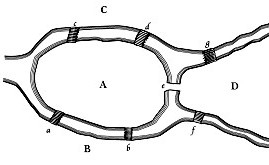
\includegraphics[scale=.75]{fig/images}
  \captionsetup{font=footnotesize}
  \caption{Dibujo de los puentes de Königsberg}
 \end{minipage}
 \begin{minipage}[b]{.5\textwidth}
  \centering
  \begin{tikzpicture}
     \GraphInit[vstyle=Shade]
     \begin{scope}
     \tikzstyle{every node} = [draw,
                               shape          = circle,
                               ball color     = orange,
                               text           = black,
                               minimum size   = 24 pt]
     \node (A) at (0,   0){A};
     \node (B) at (0,-1.8){B};
     \node (C) at (0, 1.8){C};
     \node (D) at (4,   0){D};
     \end{scope}
     \begin{scope}
     \tikzset{EdgeStyle/.append style = {bend left}}
     \Edge[label=$b$](A)(B)
     \Edge[label=$c$](A)(C)
     \end{scope}
     \begin{scope}
     \tikzset{EdgeStyle/.append style = {bend right}}
     \Edge[label=$a$](A)(B)
     \Edge[label=$d$](A)(C)
     \end{scope}
     \Edge[label=$f$](B)(D)
     \Edge[label=$e$](A)(D)
     \Edge[label=$g$](C)(D)
  \end{tikzpicture}
  \captionsetup{font=footnotesize}
  \caption{Modelo de los puentes de Königsberg}
 \end{minipage}
\end{figure}

Desde entonces, se ha ido desarrollando esta metodología hasta convertise en
los últimos años en una herramienta importante en áreas del conocimiento muy
variadas como, por ejemplo: la Investigación Operativa, la Computación, la
Ingeniería Eléctrica, la Geografía y la Química. Es por ello que, además, se ha
erigido como una nueva disciplina matemática, que generalmente asociada a las
ramas de Topología y Álgebra.

La utilidad de los grafos se basa en su gran poder de abstracción y una
representación muy clara de cualquier relación, lo que facilita enormemente
tanto la fase de modelado como la de resolución de cualquier problema. Gracias
a la Teoría de Grafos se han desarrollado una gran variedad de algoritmos y
métodos de decisión que podemos implementar a través de lenguajes funcionales y
permiten automatizar la resolución de muchos problemas, a menudo tediosos de
resolver a mano.

\comentario{Pendiente de ampliar la introducción conforme se vaya escribiendo
  los módulos.}

\minitoc

\section{Definición de grafo}

En primer lugar, vamos a introducir terminología básica en el 
desarrollo de la Teoría de Grafos.

\begin{definicion}
  Un \textbf{grafo} $G$ es un par $(V,A)$, donde $V$ es el conjunto 
  cuyos elementos llamamos \textbf{vértices} (o \textbf{nodos}) y 
  $A$ es un conjunto cuyos elementos llamamos \textbf{aristas}. 
\end{definicion}

\begin{definicion}
  Una \textbf{arista} de un grafo $G = (V,A)$, es un conjunto de dos elementos
  de $V$. Es decir, para dos vértices $v,v'$ de $G$, $(v,v')$ y $(v',v)$
  representa la misma arista.
\end{definicion}

\begin{definicion}
  Dado un grafo $G = (V,A)$, diremos que un vértice $v \in V$ es 
  \textbf{adyacente} a $v' \in V$ si $(v',v) \in A$. 
\end{definicion}

\begin{definicion}
  Si en un grafo dirigido se permiten aristas repetidas, lo llamaremos 
  \textbf{multigrafo}. Si no se permiten, lo llamaremos 
  \textbf{grafo regular}.
\end{definicion}

\begin{nota}
  Denotaremos por $|V|$ al número de vértices y por $|A|$ al número de aristas
  del grafo $(V,A)$.
\end{nota}

\begin{ejemplo}
  Sea $G = (V,A)$ un grafo con $V = \{a,b,c,d\}$ y
  $A = \{\allowbreak(a,b), \allowbreak (a,c), \allowbreak (b,d), 
  \allowbreak (d,d)\}$.
  En este grafo, los vértices $a,d$ son adyacentes a $b$.

  \begin{center},
  \begin{tikzpicture}
  \SetVertexNoLabel
  \tikzstyle{every node} = [draw, 
                            shape = circle,
                            ball color=orange,
                            minimum size = 24pt]
  \GraphInit [vstyle = Shade]
  \node (a) at (0:1.5){a};
  \node (b) at (90:1.5){b};
  \node (c) at (180:1.5){c};
  \node (d) at (270:1.5){d};
  \Edge (a)(b)
  \Edge (a)(c)
  \Edge (b)(d)
  \Edge (d)(d);
  \end{tikzpicture}
  \end{center}
\end{ejemplo}

\section{El TAD de los grafos}

\label{sec:TAD_grafos}

En esta sección, nos planteamos la tarea de implementar las definiciones
presentadas anteriormente en un lenguaje funcional. En nuestro caso, el
lenguaje que utilizaremos será Haskell. Definiremos el Tipo Abstracto de Dato
(TAD) de los grafos y daremos algunos ejemplos de posibles representaciones de
grafos con las que podremos trabajar.

Si consideramos un grafo finito cualquiera $G = (V,A)$, podemos ordenar el
conjunto de los vértices y representarlo como $V = \{v_1, \dots, v_n\}$ con
$n = |V|$.

En primer lugar, necesitaremos crear un tipo \texttt{(Grafo)} cuya definición
sea compatible con la entidad matemática que representa y que nos permita 
definir las operaciones que necesitamos para trabajar con los grafos. 
Estas operaciones son:

\begin{code}
creaGrafo  -- [a] -> [(a,a)] -> Grafo a
vertices   -- Grafo a -> [a]
adyacentes -- Grafo a -> a -> [a]
aristaEn   -- (a,a) -> Grafo a -> Bool
aristas    -- Grafo a -> [(a,a)]
\end{code}
donde:

\begin{itemize}
\item \texttt{(creaGrafo vs as)} es un grafo tal que el conjunto de sus
  vértices  es \texttt{vs} y el de sus aristas es \texttt{as}.
\item \texttt{(vertices g)} es la lista de todos los vértices del 
  grafo \texttt{g}.
\item \texttt{(adyacentes g v)} es la lista de los vértices adyacentes
  al vértice
  \texttt{v} en el grafo \texttt{g}.
\item \texttt{(aristaEn a g)} se verifica si \texttt{a} es una arista del grafo
  \texttt{g}.
\item \texttt{(aristas g)} es la lista de las aristas del grafo \texttt{g}.
\end{itemize}

\begin{nota}
  Las funciones que aparecen en la especificación del TAD no dependen 
  de la representación que elijamos.
\end{nota}

\begin{ejemplo}

Veamos un ejemplo de creación de grafo y su representación gráfica

\begin{code}
creaGrafo [1..5] [(1,2),(1,3),(1,5),(2,4),
                  (2,5),(3,4),(3,5),(4,5)]
\end{code}

\begin{center}
\begin{tikzpicture}
   \tikzstyle{every node} = [draw, 
                             shape        = circle,
                             ball color   = orange,
                             minimum size = 24pt]
   \GraphInit[vstyle=Shade]
   \node (v0) at (4*72:1.5) {1};
   \node (v1) at (   0:1.5) {2};
   \node (v2) at (  72:1.5) {3};
   \node (v3) at (2*72:1.5) {4};
   \node (v4) at (3*72:1.5) {5};
   \Edge(v0)(v1)
   \Edge(v0)(v2)
   \Edge(v0)(v4)
   \Edge(v1)(v3)
   \Edge(v1)(v4)
   \Edge(v2)(v3)
   \Edge(v2)(v4)
   \Edge(v3)(v4);
\end{tikzpicture}
\end{center}
\end{ejemplo}

\subsection{Grafos como listas de aristas}

\entrada{GrafoConListaDeAristas}

\section{Generador de grafos}

\entrada{GeneradorGrafos}

\section{Ejemplos de grafos}

\entrada{EjemplosGrafos}

\section{Definiciones y propiedades}

\entrada{DefinicionesYPropiedades}

\section{Morfismos de grafos}

\entrada{Morfismos}

\section{Caminos en grafos}

\entrada{Caminos}

\section{Conectividad de los grafos}

\entrada{Conectividad}

%%% Local Variables:
%%% mode: latex
%%% TeX-master: "MD_en_Haskell"
%%% End:

\chapter{Matrices asociadas a grafos}

En este capítulo se definirán algunas representaciones de grafos como matrices,
se comprobarán sus propiedades y volveremos a definir algunos conceptos del 
capítulo \ref{cap:Intro_Grafos} ahora utilizando matrices.

Para elaborar el contenido del capítulo utilizaré el segundo tema del trabajo
fin de grado de Fco. Javier Franco Galvín: \textit{Aspectos algebraicos en
Teoría de Grafos} (\cite{Franco-tfg}). En el trabajo, el autor introduce los 
conceptos de \textit{matriz de adyacencia}, \textit{matriz de incidencia} y 
otras matrices asociadas a grafos.

\section{Generador de grafos simples}

\entrada{GeneradorGrafosSimples}

\section{Matrices de adyacencia}

%%% Local Variables:
%%% mode: latex
%%% TeX-master: "MD_en_Haskell"
%%% End:

\chapter{Apéndices}

\section {Sistemas utilizados}

El desarrollo de mi Trabajo de Fin de Grado requería de una infraestructura
técnica que he tenido que trabajar antes de comenzar a desarrollar el contenido.
A continuación, voy a nombrar y comentar los sistemas y paquetes que he 
utilizado a lo largo del proyecto. 

\begin{itemize}
  \item \textbf{Ubuntu como sistema operativo.} El primer paso fue instalar
    \textit{Ubuntu} en mi ordenador portátil personal. Para ello, seguí las 
    recomendaciones de mi compañero Eduardo Paluzo, quien ya lo había hecho 
    antes. 

    Primero, me descargué la imagen del sistema \textit{Ubuntu 16.04 LTS} (para 
    procesador de 64 bits) desde la 
    \href{http://www.ubuntu.com/download/desktop}
    {página de descargas de Ubuntu}
    \footnote{\url{http://www.ubuntu.com/download/desktop}} y también la
    herramienta 
    \href{http://www.linuxliveusb.com/}
    {LinuxLive USB Creator}
    \footnote{\url{http://www.linuxliveusb.com/}} 
    que transformaría mi pendrive en una unidad USB Booteable cargada con la
    imagen de Ubuntu. Una vez tuve la unidad USB preparada, procedí a instalar
    el nuevo sistema: apagué el dispositivo y al encenderlo entré en el  
    \texttt{Boot Menu} de la  \texttt{BIOS} del portátil para arrancar desde el
    Pendrive en vez de hacerlo desde el disco duro. 
    Automáticamente, comenzó la instalación de  \textit{Ubuntu} y solo tuve que
    seguir las instrucciones del asistente para montar Ubuntu manteniendo además
    \textit{Windows 10}, que era el sistema operativo con el que había estado 
    trabajando hasta ese momento.
    
    El resultado fue un poco agridulce, pues la instalación de Ubuntu se había
    realizado con éxito, sin embargo, al intentar arrancar  \textit{Windows} 
    desde la nueva \texttt{GRUB}, me daba un error al cargar la imagen del 
    sistema. Después de buscar el error que me aparecía en varios foros, 
    encontré una solución a mi problema: deshabilité el  \texttt{Security Boot} 
    desde la  \texttt{BIOS} y pude volver a arrancar  \textit{Windows 10} con 
    normalidad.

  \item \textbf{\LaTeX{} como sistema de composición de textos.} La distribución
    de \LaTeX{},\textit{Tex Live}, como la mayoría de software que he utilizado,
    la descargué utilizando el \textit{Gestor de Paquetes Synaptic}.
    Anteriormente, sólo había utilizado  \textit{TexMaker} como editor de 
    \LaTeX{} así que fue el primero que descargué. Más tarde, mi tutor José 
    Antonio me sugirió que mejor descargara el paquete \textit{AUCTex}, pues me
    permitiría trabajar con archivos \TeX{} desde el editor \textit{Emacs}, así
    lo hice y es el que he utilizado para redactar el trabajo. Además de los que
    me recomendaba el gestor, solo he tenido que descargarme el paquete 
    \textit{spanish} de \textit{babel} para poder componer el trabajo, pues
    el paquete \textit{Tikz}, que he utilizado para representar los grafos,
    venía incluido en las sugerencias de \textit{Synaptic}.

  \item \textbf{Haskell como lenguaje de programación.} Ya había trabajado 
    anteriormente con este lenguaje en el grado y sabía que sólo tenía que 
    descargarme la plataforma de \textit{Haskell} y podría trabajar con el 
    editor \textit{Emacs}. Seguí las indicaciones que se dan a los estudiantes
    de primer curso en la 
    \href{http://www.cs.us.es/~jalonso/cursos/i1m-15/sistemas.php}
    {página del Dpto. de Ciencias de la Computación e Inteligencia Artificial}
    \footnote{\url{http://www.cs.us.es/~jalonso/cursos/i1m-15/sistemas.php}}
    y me descargué los paquetes \textit{haskell-platform} y 
    \textit{haskell-mode} desde el \textit{Gestor de Paquetes Synaptic}. La 
    versión de la plataforma de \textit{Haskell} con la que he trabajado
    es la \textit{2014.2.0.0.debian2} y la del compilador \textit{GHC} la
    \textit{7.10.3-7}.


  \item \textbf{Dropbox como sistema de almacenamiento compartido.} Ya había 
    trabajado con \textit{Dropbox} en el pasado, así que crear una carpeta 
    compartida con mis tutores no fue ningún problema; sin embargo, al estar
    \textit{Dropbox} sujeto a software no libre, no me resultó tan sencillo
    instalarlo en mi nuevo sistema. En primer lugar, intenté hacerlo 
    directamente desde \textit{Ubuntu Software}, que intentó instalar 
    \textit{Dropbox Nautilus} y abrió dos instalaciones en paralelo. Se quedó 
    colgado el ordenador, así que maté los procesos de instalación activos,
    reinicié el sistema y me descargué directamente el paquete de instalación
    desde la 
    \href{https://www.dropbox.com/es/install?os=lnx}
    {página de descargas de Dropbox}
    \footnote{\url{https://www.dropbox.com/es/install?os=lnx}} y lo ejecuté
    desde la terminal.
  \item \textbf{Git como sistema remoto de control de versiones.} Era la 
    primera vez que trabajaba con \textit{Git} y me costó bastante adaptarme.
    Mi tutor José Antonio y mi compañero Eduardo Paluzo me ayudaron mucho e
    hicieron el proceso de adaptación mucho más ágil. 
    El manual que Eduardo ha redactado y presenta en su Trabajo Fin de Grado
    me ha sido muy útil; es una pequeña guía que cualquier interesado en el
    empleo de \textit{Git} puede utilizar como introducción.
    La instalación no resultó complicada: a través del \textit{Gestor de 
    Paquetes Synaptic} me descargué el paquete \textit{elpa-magit} y todos
    los demás paquetes necesarios para trabajar con \textit{Git} en mi
    portátil usando el editor \textit{Emacs}.
    Eduardo me ayudó a crear el repositorio \textit{MDenHaskell} en la 
    plataforma \textit{GitHub} y clonarlo en mi ordenador personal. Dicho
    repositorio contiene el total del trabajo y se almacena de forma pública.
    La versión de \textit{Magit} que utilizo es la \textit{2.5.0-2}
\end{itemize}

\section{Mapa de decisiones de diseño en conjuntos}

Una vez comenzado el trabajo y habiendo hecho ya varias secciones acerca de la
Teoría de Grafos, se puso de manifiesto la conveniencia de crear nuevos 
capítulos introduciendo conceptos de la Teoría de Conjuntos y las relaciones
que se pueden presentar entre sus elementos. 

Haskell tiene una librería específica para conjuntos: \texttt{Data.Set}, sin
embargo, no es tan intuitiva ni tan eficiente como la de listas 
(\texttt{Data.List}). A lo largo del proyecto he creado un módulo que permite
trabajar con conjuntos utilizando tanto su representación como listas ordenadas
sin elementos repetidos como su representación como listas sin elementos
repetidos. Dicho módulo se llama \texttt{Conjuntos} y lo presento en el primer
capítulo del Trabajo \ref{cap:Conjuntos}.

\section{Mapa de decisiones de diseño en grafos}

Al comienzo del proyecto, la idea era que las primeras representaciones con las
que trabajara fueran las de \textit{grafos como vectores de adyacencia} y 
\textit{grafos como matrices de adyacencia} que se utilizan en Informática en el
primer curso del Grado, con las que ya había trabajado y estaba familiarizada. 

Las definiciones de Informática están pensadas para grafos ponderados (dirigidos
o no según se eligiera), mientras que en Matemática Discreta apenas se usan 
grafos dirigidos o ponderados; por tanto, el primer cambio en la representación 
utilizada fue simplificar las definiciones de modo que solo trabajáramos con
grafos no dirigidos y no ponderados, pero manteniendo las estructuras vectorial
y matricial que mantenían la eficiencia. 

Las representaciones que utilizan \textit{arrays} en \textit{Haskell} son muy
restrictivas, pues solo admiten vectores y matrices que se puedan indexar, lo
que hace muy complicados todos los algoritmos que impliquen algún cambio en los
vértices de los grafos y, además, no permite trabajar con todos los tipos de
vértices que pudiéramos desear. Decidimos volver a cambiar la representación, y
esta vez nos decantamos por la representación de \textit{grafos como listas de
aristas}, perdiendo en eficiencia pero ganando mucho en flexibilidad de
escritura.

Por último mis tutores sugirieron dar una representación de los grafos
mediante sus matrices de adyacencia y comprobar la equivalencia de las
definiciones que ya había hecho en otros módulos con las dadas para esta 
representación. Para ello he trabajado con la librería \texttt{Data.Matrix} 
de \textit{Haskell}.

%%% Local Variables:
%%% mode: latex
%%% TeX-master: "MD_en_Haskell"
%%% End:


%%%%%%%%%%%%%%%%%%%%%%%%%%%%%%%%%%%%%%%%%%%%%%%%%%%%%%%%%%%%%%%%%%%%%%%%%%%%%%%
%%  Bibliografía                                                            %%
%%%%%%%%%%%%%%%%%%%%%%%%%%%%%%%%%%%%%%%%%%%%%%%%%%%%%%%%%%%%%%%%%%%%%%%%%%%%%%%

\addcontentsline{toc}{chapter}{Bibliografía}
\bibliographystyle{abbrv}
\bibliography{MD_en_Haskell}

%%%%%%%%%%%%%%%%%%%%%%%%%%%%%%%%%%%%%%%%%%%%%%%%%%%%%%%%%%%%%%%%%%%%%%%%%%%%%%%
%%  Índice                                                                  %%
%%%%%%%%%%%%%%%%%%%%%%%%%%%%%%%%%%%%%%%%%%%%%%%%%%%%%%%%%%%%%%%%%%%%%%%%%%%%%%%

\addcontentsline{toc}{chapter}{Indice de definiciones}

\printindex

%%%%%%%%%%%%%%%%%%%%%%%%%%%%%%%%%%%%%%%%%%%%%%%%%%%%%%%%%%%%%%%%%%%%%%%%%%%%%%%
%% § Pendientes                                                              %%
%%%%%%%%%%%%%%%%%%%%%%%%%%%%%%%%%%%%%%%%%%%%%%%%%%%%%%%%%%%%%%%%%%%%%%%%%%%%%%%

%%\todototoc
%%\listoftodos

\end{document}



%%% Local Variables:
%%% mode: latex
%%% TeX-master: t
%%% End:
